\documentclass{article}
\usepackage[utf8]{inputenc}
\title{Lesson 5 - Discrete Mathematics}
\author{Matt Chung}
\date{August 14 2017}
\usepackage{tikz}
\usepackage{verbatim}
\usetikzlibrary{calc}

\begin{document}
\maketitle

\section{}

\begin{center}
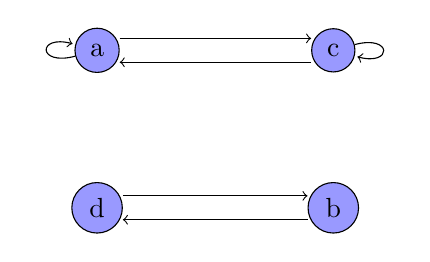
\begin{tikzpicture}

\node[circle, fill=blue!40!white!, draw=black] (a) at (0,0) {a};

\node[circle, fill=blue!40!white!, draw=black] (c) at ($(a) + (3, 0)$) {c};

\node[circle, fill=blue!40!white!, draw=black] (b) at ($(c) + (0, -2)$) {b};

\node[circle, fill=blue!40!white!, draw=black] (d) at ($(a) + (0, -2)$) {d};

\draw[->] ([yshift=1ex]a.east) -- ([yshift=1ex]c.west);
\draw[->] ([yshift=-1ex]c.west) -- ([yshift=-1ex]a.east);

\draw[->] ([yshift=1ex]d.east) -- ([yshift=1ex]b.west);
\draw[->] ([yshift=-1ex]b.west) -- ([yshift=-1ex]d.east);

\path (a) edge [loop left] node {} (a);
\path (c) edge [loop right] node {} (c);

\end{tikzpicture}
\end{center}

\section{}

${(1,x), (1,y), (4,x), (4,y), (5,x), (2,z), (5,z), (3,z)}$

The way I solved this was by drawing a bipartite graph, creating three columns, connecting the left most column to the center column (i.e. $S$), the center to the right most (i.e. $R$). 

\section{}

$R1 \cup R2: (1,2), (1,3), (1,5), (1,6), (2,1), (3,6), (4,2), (5,6), (6,2), (6,3), (6,6)$\\
$R1 \cap R2: (1,2)$

Below are the sets and to solve the former, we get the union (i.e. appear in at least one of the relations); the latter, we get the intersection (i.e. elements in both sets).

$R1 = (1,2), (1,3), (1,5), (2,1), (6,6)$

$R2 = (1,2), (1,6), (3,6), (4,2), (5,6), (6,2), (6,3)$

\section{}

\textbf{Solution:} Irreflexive, symmetric.

Here's our set: ${(1,2), (2,1), (2,3), (3,2), (3,4), (4,3), (4,5), (5,4), (5,1), (1,5)}$

This question asks if the relation satisfies any of the properties: reflexive, irreflexive, symmetric, and so on. Let's list each of these properties out and, one by one, compare the items in each set.

Let's start with reflexive. For example, let's say we have the items $\{1,2,3\}$. In order to be reflexive, we need each element to relate to itself; in order words: ${(1,1), (2,2), (3,3)}$. But, in this example, we \textbf{do not} the corresponding, elements do not exist. Therefore, this relation does not exhibit a reflexive property. Instead, we categorize this relation as irreflexive, no item in the set related to itself. We have ${1,2,3,4,5}$ but do not have any of the following: ${(1,1), (2,2), (3,3), (4, 4), (5, 5)}$

Now, how about symmetric? In order to be symmetric, even item element in the set must contain an opposite element. Let me elaborate: if we have an element $(a,b)$ in the set, we need to have the element $(b, a)$. Do we have that in our relation? Yes, we do. Let's pick out the items in the set and start with the first element: ${(1,2)}$. $1$ is $a$ and $2$ is $b$. 

What about antisymmetric? To be antisymmetric, all elements in our relation must be the same. For example, this would be antisymmetric: $\{(1,1), (2,2), (3,3)\}$. In our case, this is not the case. We have objects that are not the same. Therefore, our relation does not exhibit the antisymmetric property.

Next up: transitive property. A transitive property goes something like this: $(a,b), (b,c), (a,c)$. For example, if we have $(1,2), (2,3)$, what do we need to fulfill this transitive relationship? Simple: $(1,3)$. But, is that the case with our relation? No because we have $(1,2)$ and $(2,3)$ but do not have the needed element: $(1,3)$

\section{}

$M(A,B): A \cap B = \emptyset$

\begin{comment}
What does this mean in English?

Okay, I almost screwed up this entire problem, thinking that we are trying to prove that we produce a non-empty set, when in reality, we are trying to produce an empty set.

Like the previous problem, let's work through each of the properties, one at a time.

I'm double screwed. I think we are stipulating that that the relation will always produce an empty set.

So the question now is, what examples can we provide where $A \cap B$ does not produce an empty set (i.e. $\emptyset$)

How do we tell if it's symmetric. We need to have all elements in A to be present in the set B.

\end{comment}

\begin{itemize}
    \item $M$ is not reflexive. For example, let's say $A = \{1,2\}$ and $B = \{3,2\}$.  $A M A$ (i.e. $\{1,2\} \cap \{1,2\}$) produces the set $\{1,2\}$, not $\emptyset$.
    \item $M$ is irreflexive since every set unioned with itself will produce the same set, never an $\emptyset$.
    \item $M$ is not symmetric because if there are any elements in both sets, we produce a set that is not an empty set. For example, $\{1\}M\{1,2\}$ produces $\{1\}$, not an empty set.
    \item $M$ is not antisymmetric. $\{1,2,3\} \cap \{4,5,6\}$ produces an empty set. So does $\{4,5,6\} \cap \{1,2,3\}$. Both produce an empty set (i.e. $\emptyset$). But the sets are not the same. In fact, they can never be the same since that produces a non empty set.
    \item $M$ is not transitive. For example, let's stipulate the following: $A = \{1,2,3\}; B = \{4,5,6\}; C= \{1,2,3\}$. Although $A M B$ is True, and $B M C$ is true, $A M C$ would not be true, because we would produce a set of $\{1,2,3\}$, a non-empty set, making the relation false.
\end{itemize}

\section{}

$A = \emptyset$ and the empty relation $E = \emptyset$, on $A$.

\begin{itemize}
    \item reflexive is true it satisfies the following condition: $\forall a \in A, aRa$. $\forall x(x \in \emptyset \to (x,x) \in E)$ since the hypothesis is always false, the entire predicate will always be true.
    \item irreflexive is false because because we need to negate the following expression: $\forall x(x \in \emptyset \to (x,x) \in E)$. Since we already discovered that this prediate will always yield True, then the negation of it will always yield False.
    \item symmetric is true. The condition we are checking for is: $(x,y) \in \emptyset \to (y,x) \in E$. And since the hypothesis is false—there are no items in the empty set—then the entire predicate yields true. Therefore, this is true.
    \item antisymmetric is false. There are two conditions that must be satisified: $(x,y) \in \emptyset \land (y,x) \in \emptyset$. And since both expression will always be false, we can never get $x = y$.
    \item transitive is true. For transitive relations, we would need a series of expressions to all be true: $((a,b) \in E) \land ((b,c) \in E) \to (a,c) \in E$ 
\end{itemize}
\end{document}